\documentclass[addpoints,10pt]{exam}

\usepackage{amsmath,amsthm,enumitem,wrapfig,amsfonts,mathtools}
\usepackage[mathscr]{euscript}
\usepackage[super]{nth}

\usepackage{geometry}
\usepackage[T1]{fontenc} % Use 8-bit encoding that has 256 glyphs
\renewcommand{\rmdefault}{ptm} %Change the Front Family from the default(cmr) to ptm(Times)
\usepackage{amsmath,amsfonts,amsthm,amssymb} % Math packages
\usepackage{bm}
\usepackage{mathptmx}
\usepackage{graphicx}
\usepackage{sectsty} % Allows customizing section commands
% \allsectionsfont{\centering} % Make all sections centered, the default font and small caps

\theoremstyle{plain}
\newtheorem{thm}{\protect\theoremname}
  \theoremstyle{definition}
  \newtheorem{prob}[thm]{Problem}
  \newtheorem*{problem*}{Open Problem}
  \theoremstyle{plain}
  \newtheorem{conjecture}[thm]{Conjecture}
  \theoremstyle{plain}
  \newtheorem{lem}[thm]{Lemma}
  \newtheorem{obs}[thm]{Observation}
  \newtheorem{cor}[thm]{Corollary}
  \theoremstyle{definition}
\newtheorem{definition}[thm]{Definition}

\newcommand{\horrule}[1]{\rule{\linewidth}{#1}}
\newcommand{\kk}{\ensuremath{\Bbbk}} 
\newcommand{\CC}{\ensuremath{\mathbb{C}}}
\newcommand{\FF}{\ensuremath{\mathbb{F}}}
\newcommand{\NN}{\ensuremath{\mathbb{N}}}
\newcommand{\QQ}{\ensuremath{\mathbb{Q}}} 
\newcommand{\RR}{\ensuremath{\mathbb{R}}} 
\newcommand{\ZZ}{\ensuremath{\mathbb{Z}}}
\newcommand{\MM}{\ensuremath{\mathcal{M}}}
\newcommand{\TT}{\ensuremath{\mathcal{T}}}
\newcommand{\BB}{\ensuremath{\mathcal{B}}}
\newcommand{\VV}{\ensuremath{\mathcal{V}}}
\newcommand{\WW}{\ensuremath{\mathcal{W}}}
\newcommand{\UU}{\ensuremath{\mathcal{U}}}
%MUDAC
\newcommand{\EE}{\ensuremath{\mathcal{F}}}
\newcommand{\YY}{\ensuremath{\mathcal{Y}}}
\newcommand{\II}{\ensuremath{\mathcal{I}}}

\newcommand{\sm}{\char`\\}

\DeclareMathOperator{\diag}{diag}

\makeatletter
\renewcommand*\env@matrix[1][*\c@MaxMatrixCols c]{%
  \hskip -\arraycolsep
  \let\@ifnextchar\new@ifnextchar
  \array{#1}}
\makeatother

\def\env@matrix{\hskip -\arraycolsep
  \let\@ifnextchar\new@ifnextchar
  \array{*\c@MaxMatrixCols c}}


\usepackage{tikz}
\usepackage{caption}
\usetikzlibrary{arrows.meta} %arrow styles
\definecolor{Purple}{RGB}{153,51,255} %purple
\definecolor{lPurple}{RGB}{200,150,255} %light purple


  

%%% Formatting: Page Header
\newcommand{\StudentName}{G04}
\newcommand{\AssignmentName}{Model}
\newcommand{\CourseName}{MUDAC 2024}


\pagestyle{headandfoot}
\runningheadrule
\firstpageheadrule
\firstpageheader{\CourseName}{\StudentName}{\AssignmentName}
\runningheader{\CourseName}{\StudentName}{\AssignmentName}
\firstpagefooter{}{\thepage}{}
\runningfooter{}{\thepage}{}

\printanswers

\DeclareMathAlphabet{\mathcal}{OMS}{cmsy}{m}{n}

\usepackage{parskip}

\begin{document}

We define the following raw variables over each region of land $\lambda_{i}\in \lambda$ in some region of land in Minnesota where $\lambda$ is a land partition of Minnesota according to some rule $(\text{street, neighborhood,}\hdots\text{, city, county, district,}\hdots)$ and $i\in [1,|\lambda|]\cap \NN$. ex.) $\lambda = \{\text{Ramsey, Anoka, St. Louis,}\hdots\}$ is a partition of Minnesota into counties. 
\begin{align*}
&F_{i}:= \text{average fuel cost per operation (american Dollars)}\\& W_{i}:= \text{total river area (acres)}\\ &T_{i}:= \text{total road miles (Combining several categories)}\\ &Y_{i}:= \text{average yield of corn ,sugarbeets ,soy, other grains (bushels/acre)}\\ &N_{i}:= \frac{\text{Nitrogen needed}}{\text{Crop Production Index}}\;\text{(N/cpi)}
\end{align*}

Normalized Variables: $\hat{F}_{i}, \hat{T}_{i}, \hat{Y}_{i}, \hat{N}_{i}, \hat{W}_{i}$


\begin{figure}[ht]
  \centering
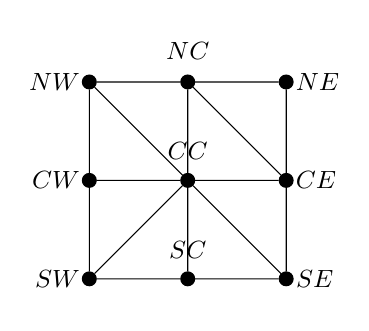
\begin{tikzpicture}[scale=1.25]
  \tikzset{
every label/.append style={font=\small},
every node/.style={
  draw,
  circle,
  fill=black,
  minimum size=5pt,
  inner sep=0pt
}
}
  %row 1 nodes
  \draw (0,0) node (NW) [label=left:{$NW$}] {};
  \draw (1,0) node (NC) [label=north:{$NC$}] {};
  \draw (2,0) node (NE) [label=right:{$NE$}] {};
  %row 2
  \draw (0,-1) node (CW) [label=left:{$CW$}] {};
  \draw (1,-1) node (CC) [label=north:{$CC$}] {};
  \draw (2,-1) node (CE) [label=right:{$CE$}] {};
  %row 3
  \draw (0,-2) node (SW) [label=left:{$SW$}] {};
  \draw (1,-2) node (SC) [label=north:{$SC$}] {};
  \draw (2,-2) node (SE) [label=right:{$SE$}] {};

  %edges
  \draw (NW)--(CW)--(SW)--(SC)--(SE)--(CE)--(NE)--(NC)--(NW){};
  \draw (SW)--(CC){};
  \draw (SC)--(CC){};
  \draw (SE)--(CC){};
  \draw (CE)--(CC){};
  \draw (CW)--(CC){};
  \draw (NW)--(CC){};
  \draw (NC)--(CC){};
  \draw (NC)--(CE){};

\end{tikzpicture}
\end{figure}

$\lambda=\{\lambda_{i}\in \lambda\mid i\in [1,|\lambda|]\cap \NN\}=\{SW,SC,SE,CW,CC,CE,NW,NC,NE\}$.

Now, let $f:\lambda\rightarrow \RR^{5}$ be defined by $f(\lambda_{i})=\begin{pmatrix}
  \hat{F}_{i}\\
  \hat{W}_{i}\\
  \hat{T}_{i}\\
  \hat{Y}_{i}\\
  \hat{N}_{i}\\
\end{pmatrix}$. $f$ produces a tuple containing the normalized variables for each of our districts $\lambda_{i}\in \lambda$. We know define our weight row vector as follows $w=(40,24,16,12,8)$ which scales $\hat{F}_{i}, \hat{T}_{i}, \hat{Y}_{i}, \hat{N}_{i}, \hat{W}_{i}$, respectively, which are ranked in order from most to least important out of $100\%$. These weights are order according to most significant with respect to economic feasibility. Finally, we mutliply $f(\lambda_{i})$ by $w$ from the left in order to produce a linear combination for each district, once again centered around economic feasibility, which we call it's rank $R$:
$$R(\lambda_{i})=wf(\lambda_{i})$$
For shorthand we simply relabel the nodes $1-9$ where $1$ is the highest and $9$ is the lowest. Finally, we select the highest ranking two nodes, and then try to move towards the rivers and transportation hubs and it's highest ranking neighbors as we select counties. Now we partition the district by county but this time we also move towards rivers more precisely. 

Our final result is (1) Hennepin County and (2) Cass County. Then we look for 2 acre availabilities, based on the factors listed above.

\end{document}